\section{Resolución de corto}
\begin{itemize}
    \item Ahorrar y después invertir en bienes de capital.
    \item Tienen más bienes de orden superior, ya tienen capital.
    \item El precio determina el costo.
\end{itemize}

\section{Noticia - La economía de españa está en peligro de una recesión}
\begin{itemize}
    \item Las cuentas nacionales: los países que invireten internacionalmente, \emph{\textbf{Definición de ``ingreso o egreso bruto":} es lo que ingreso o egresa.} \emph{\textbf{Definición de ``ingreso y egreso neto":} es la diferencia entre el ingreso y egreso bruto.}
    \item La prorroga de presupuesto no se actualiaza almenos que el gobierno se ponga de acuerdo. 
    \item PIM (purchasing manager index): indicador económico que se hace una encuesta a los compradores de empresas para ver si están comprando más que el mes pasado.
    \item Noticia, las condiciones para invertir se hace difícil.
\end{itemize}



\section{Discusión de clase}
\textbf{Dato*:} Se termina el tema de bienes.
\emph{\textbf{(Paréntesis:}Las empresas quiebran por que estiman precios mal. \textbf{\emph{(Ejemplo: El mercado de hule en GT, \textbf{Nos preguntamos:} ¿El proceso productivo del hule, cuánto dura?)}} Dura 5 años entonces el empresario debe especular 5 años y los acreedores que prestan a este especulador pueden estar sujetos a lo que pase en 5 años cuando esté el café\textbf{)}}

\begin{itemize}
    \item Repaso de bienes: los bienes de orden superior y de orden inferior la diferencia que tienen es mas que todo \textbf{tiempo}.
\end{itemize}

\begin{itemize}
    \item El interés es un precio, es por el tiempo, por el coste de oportunidad, etcétera.
    \[
      i_{M}= \underbrace{i_{\text{original}}}_{\text{precio del tiempo}} + \text{Prima riesgo} + \text{Prima de inflación}
    \]
    
    \item \emph{i} es el interés.
    \item \textbf{Prima de riesgo:} es como el límite interno, es una estimación de qué tan capaz de pagar devuelta el depósito y qué tanta buena fe tienes (historial de TDC). \emph{\textbf{(Paréntesis ``los bancos con nombres especializados'':}el banco industrial significa que le tiende a dar a las industrias préstamos\textbf{)}}
    \item \textbf{Prima de inflación:} La prima de inflación el porcentaged e inflación.
    \item \textbf{Prima de interés:} 
   \begin{figure}[htbp]
       \centering
       %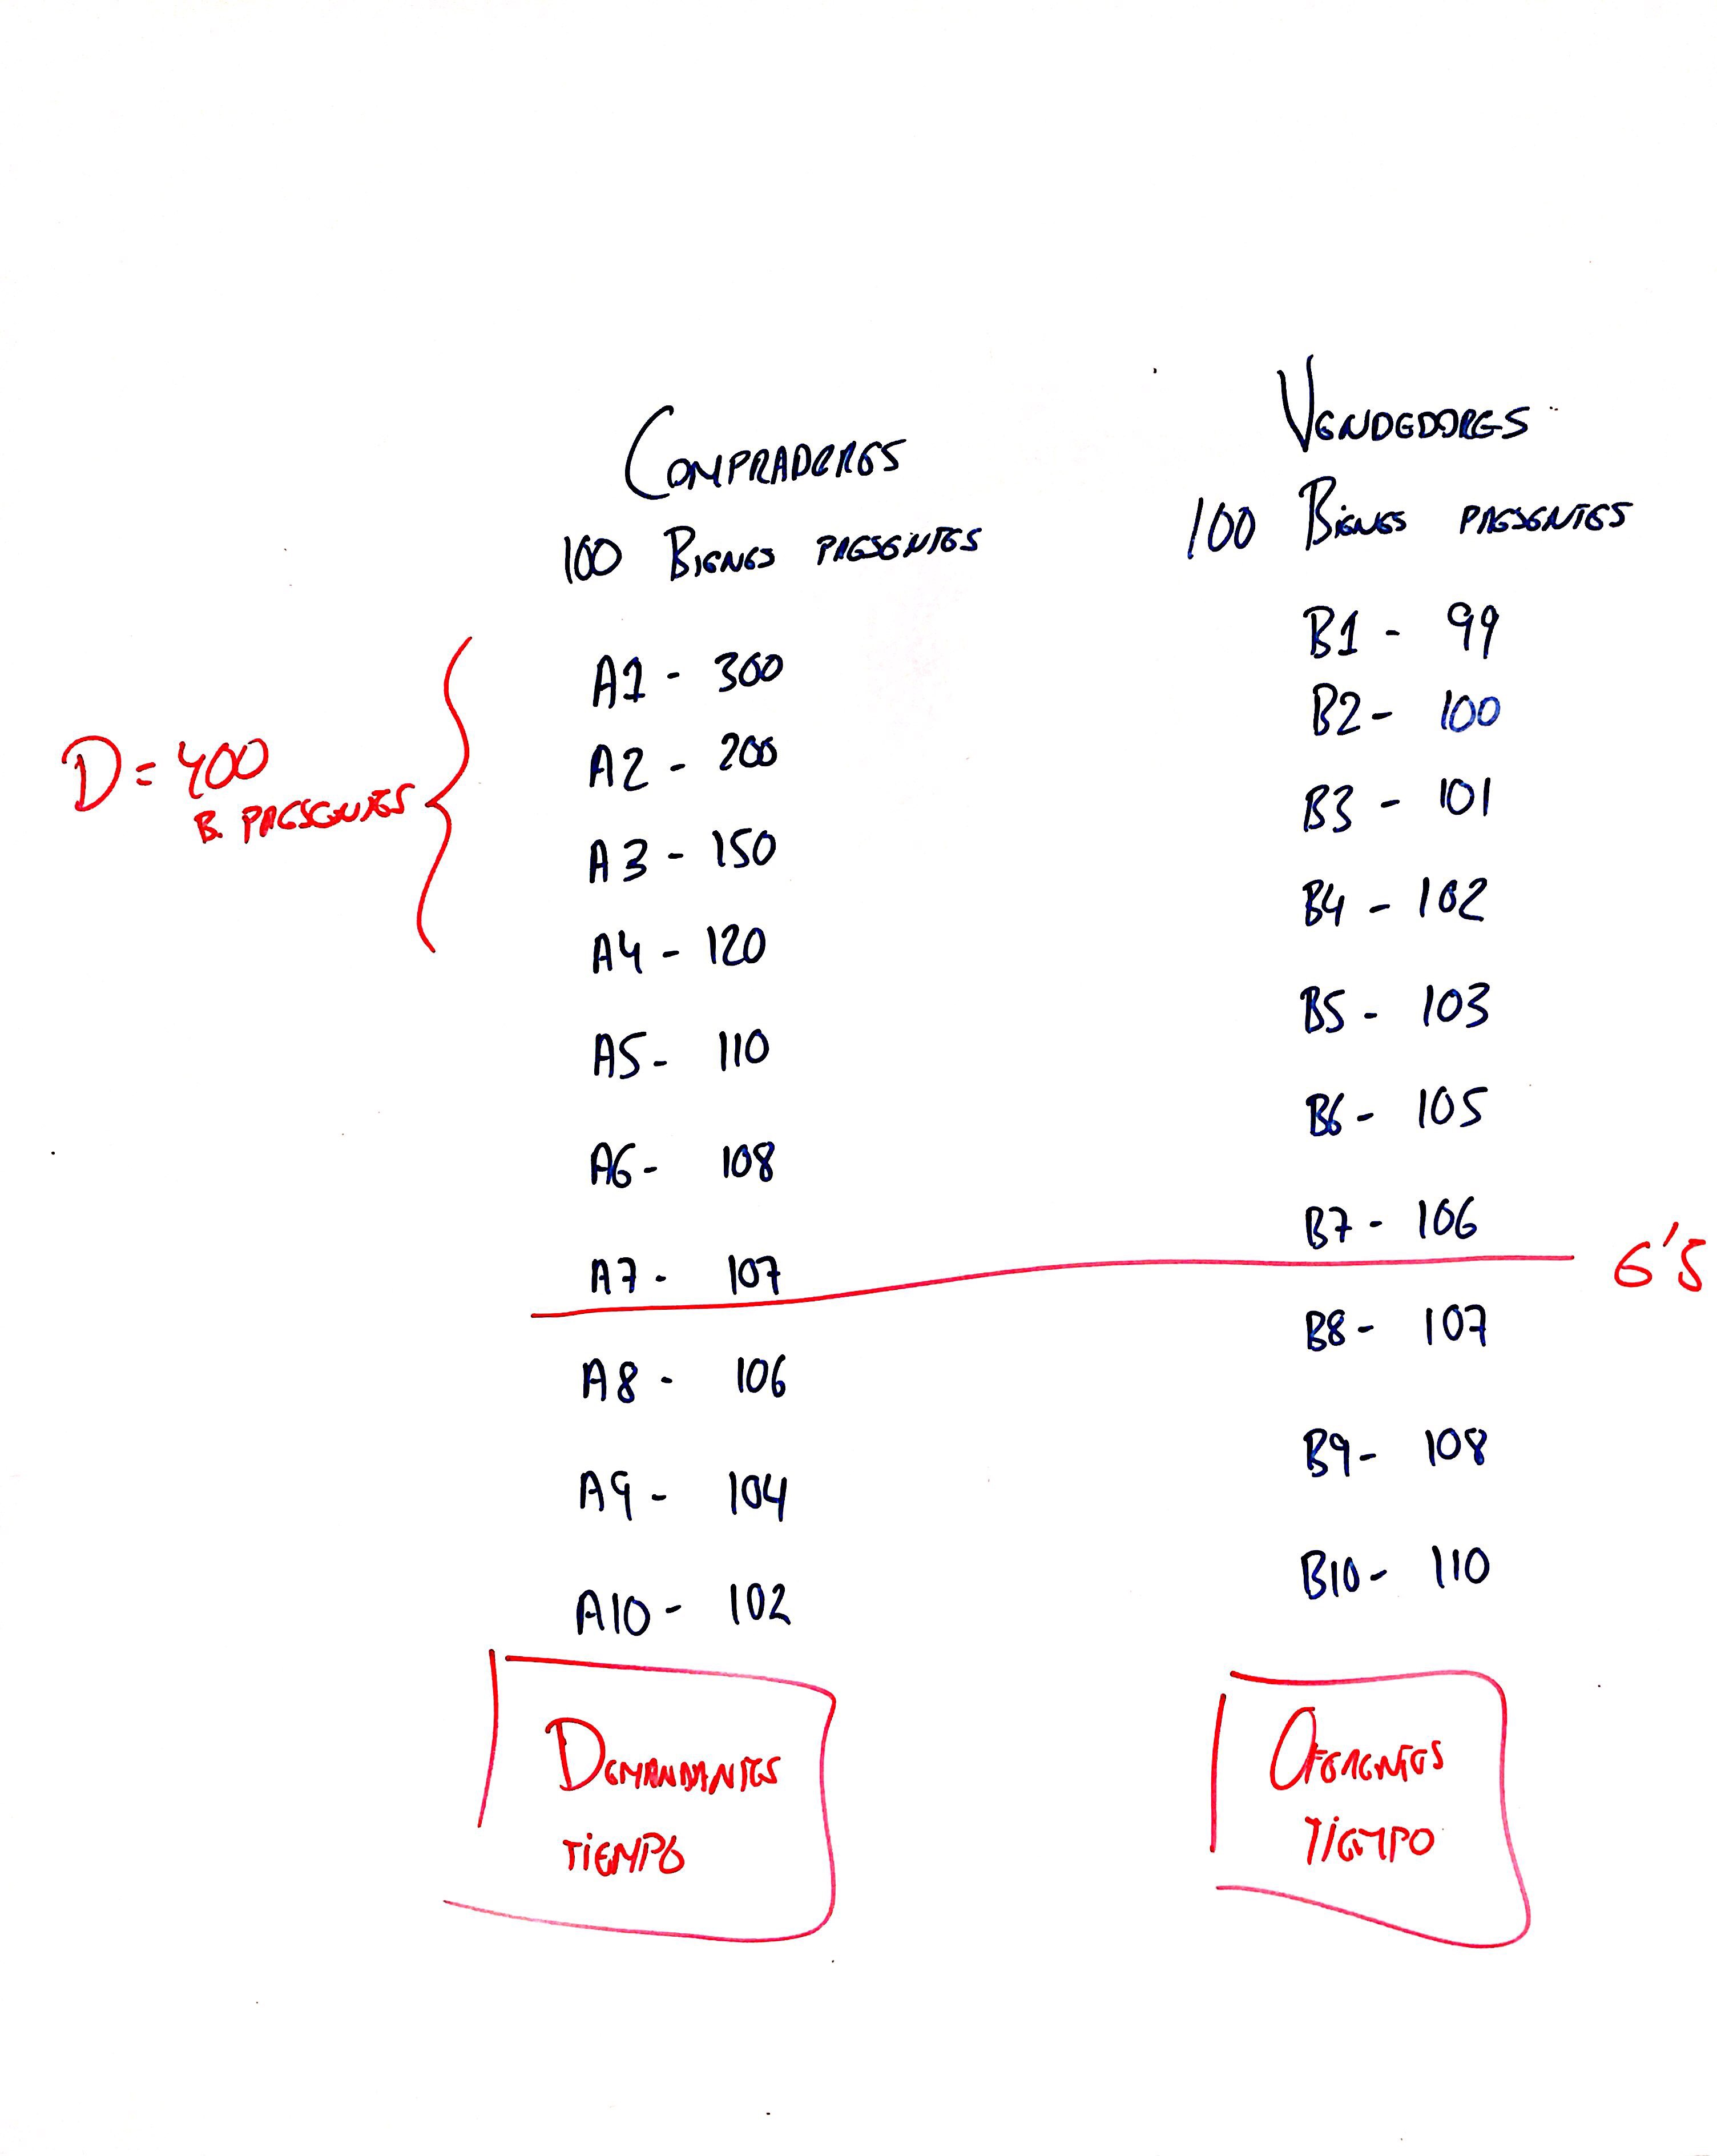
\includegraphics[width=6cm]{2019-09-04-01.jpg}
       \caption{}
       \label{}
   \end{figure} 
    
    \item La inflación beneficia al deudor, el pricipal es el estado.
    \item Veamos los oferentes del tiempo y los demandantes del tiempo.
    \begin{center}
    \begin{tabular}{ | p{5cm} | p{5cm} | }
     \hline
     Oferentes del tiempo (acreedores) & \\
     Demandantes del tiempo (deudores) & Empresarios (inversionistas) \\ 
     \hline
    \end{tabular}
    \end{center}
\end{itemize}



\subsection{Esquema de oferta y demanda de bienes presentes}
Las personas que valoran los bienes en el presentes especulando que en el futuro el bien prestado se va a aumenta respecto al interés.
\newline 
\textbf{\emph{(Ejemplo: el niño que espera 15 minutos por un nuevo dulce es un interes de 100\%)}} \emph{\textbf{(Paréntesis ``biología'':} la especie y su éxito recae en su capacidad de imaginarse en el futuro.\textbf{)}}
\begin{center}
\begin{tabular}{ | p{5cm} | p{5cm} | }
 \hline
  Compradores & Vendedores      \\
  100 Bienes presentes & 100 Bienes presentes \\ 
 \hline
    A1-300 & B1-99 \\ 
    A2-200 & B2-100 \\ 
    A3-150 & B3-101 \\ 
    A4-120 & B4-102 \\ 
    A5-110 & B5-103 \\ 
    A6-108 & B6-105 \\ 
    A7-107 & B7-106 \\ 
    A8-106 & B8-107 \\ 
    A9-104 & B9-108 \\ 
    A10-102 & B10-110 \\ 
\hline
    Demandante de tiempo & Oferentes de tiempo \\ 
\hline
\end{tabular}
\end{center}

\begin{itemize}
    \item Una onza de oro ha valido por lo general es suficiente para un mes.
    \item Mercado intertemporal.
    \item Para el interes se paga con bienes presentes respecto a la valoración subjetiva que cada uno espere recibir en el futuro.
    \item El que pone en contacto a los compradores y vendedores es el sector bancario.
\end{itemize}

\begin{figure}[htbp]
    \centering
    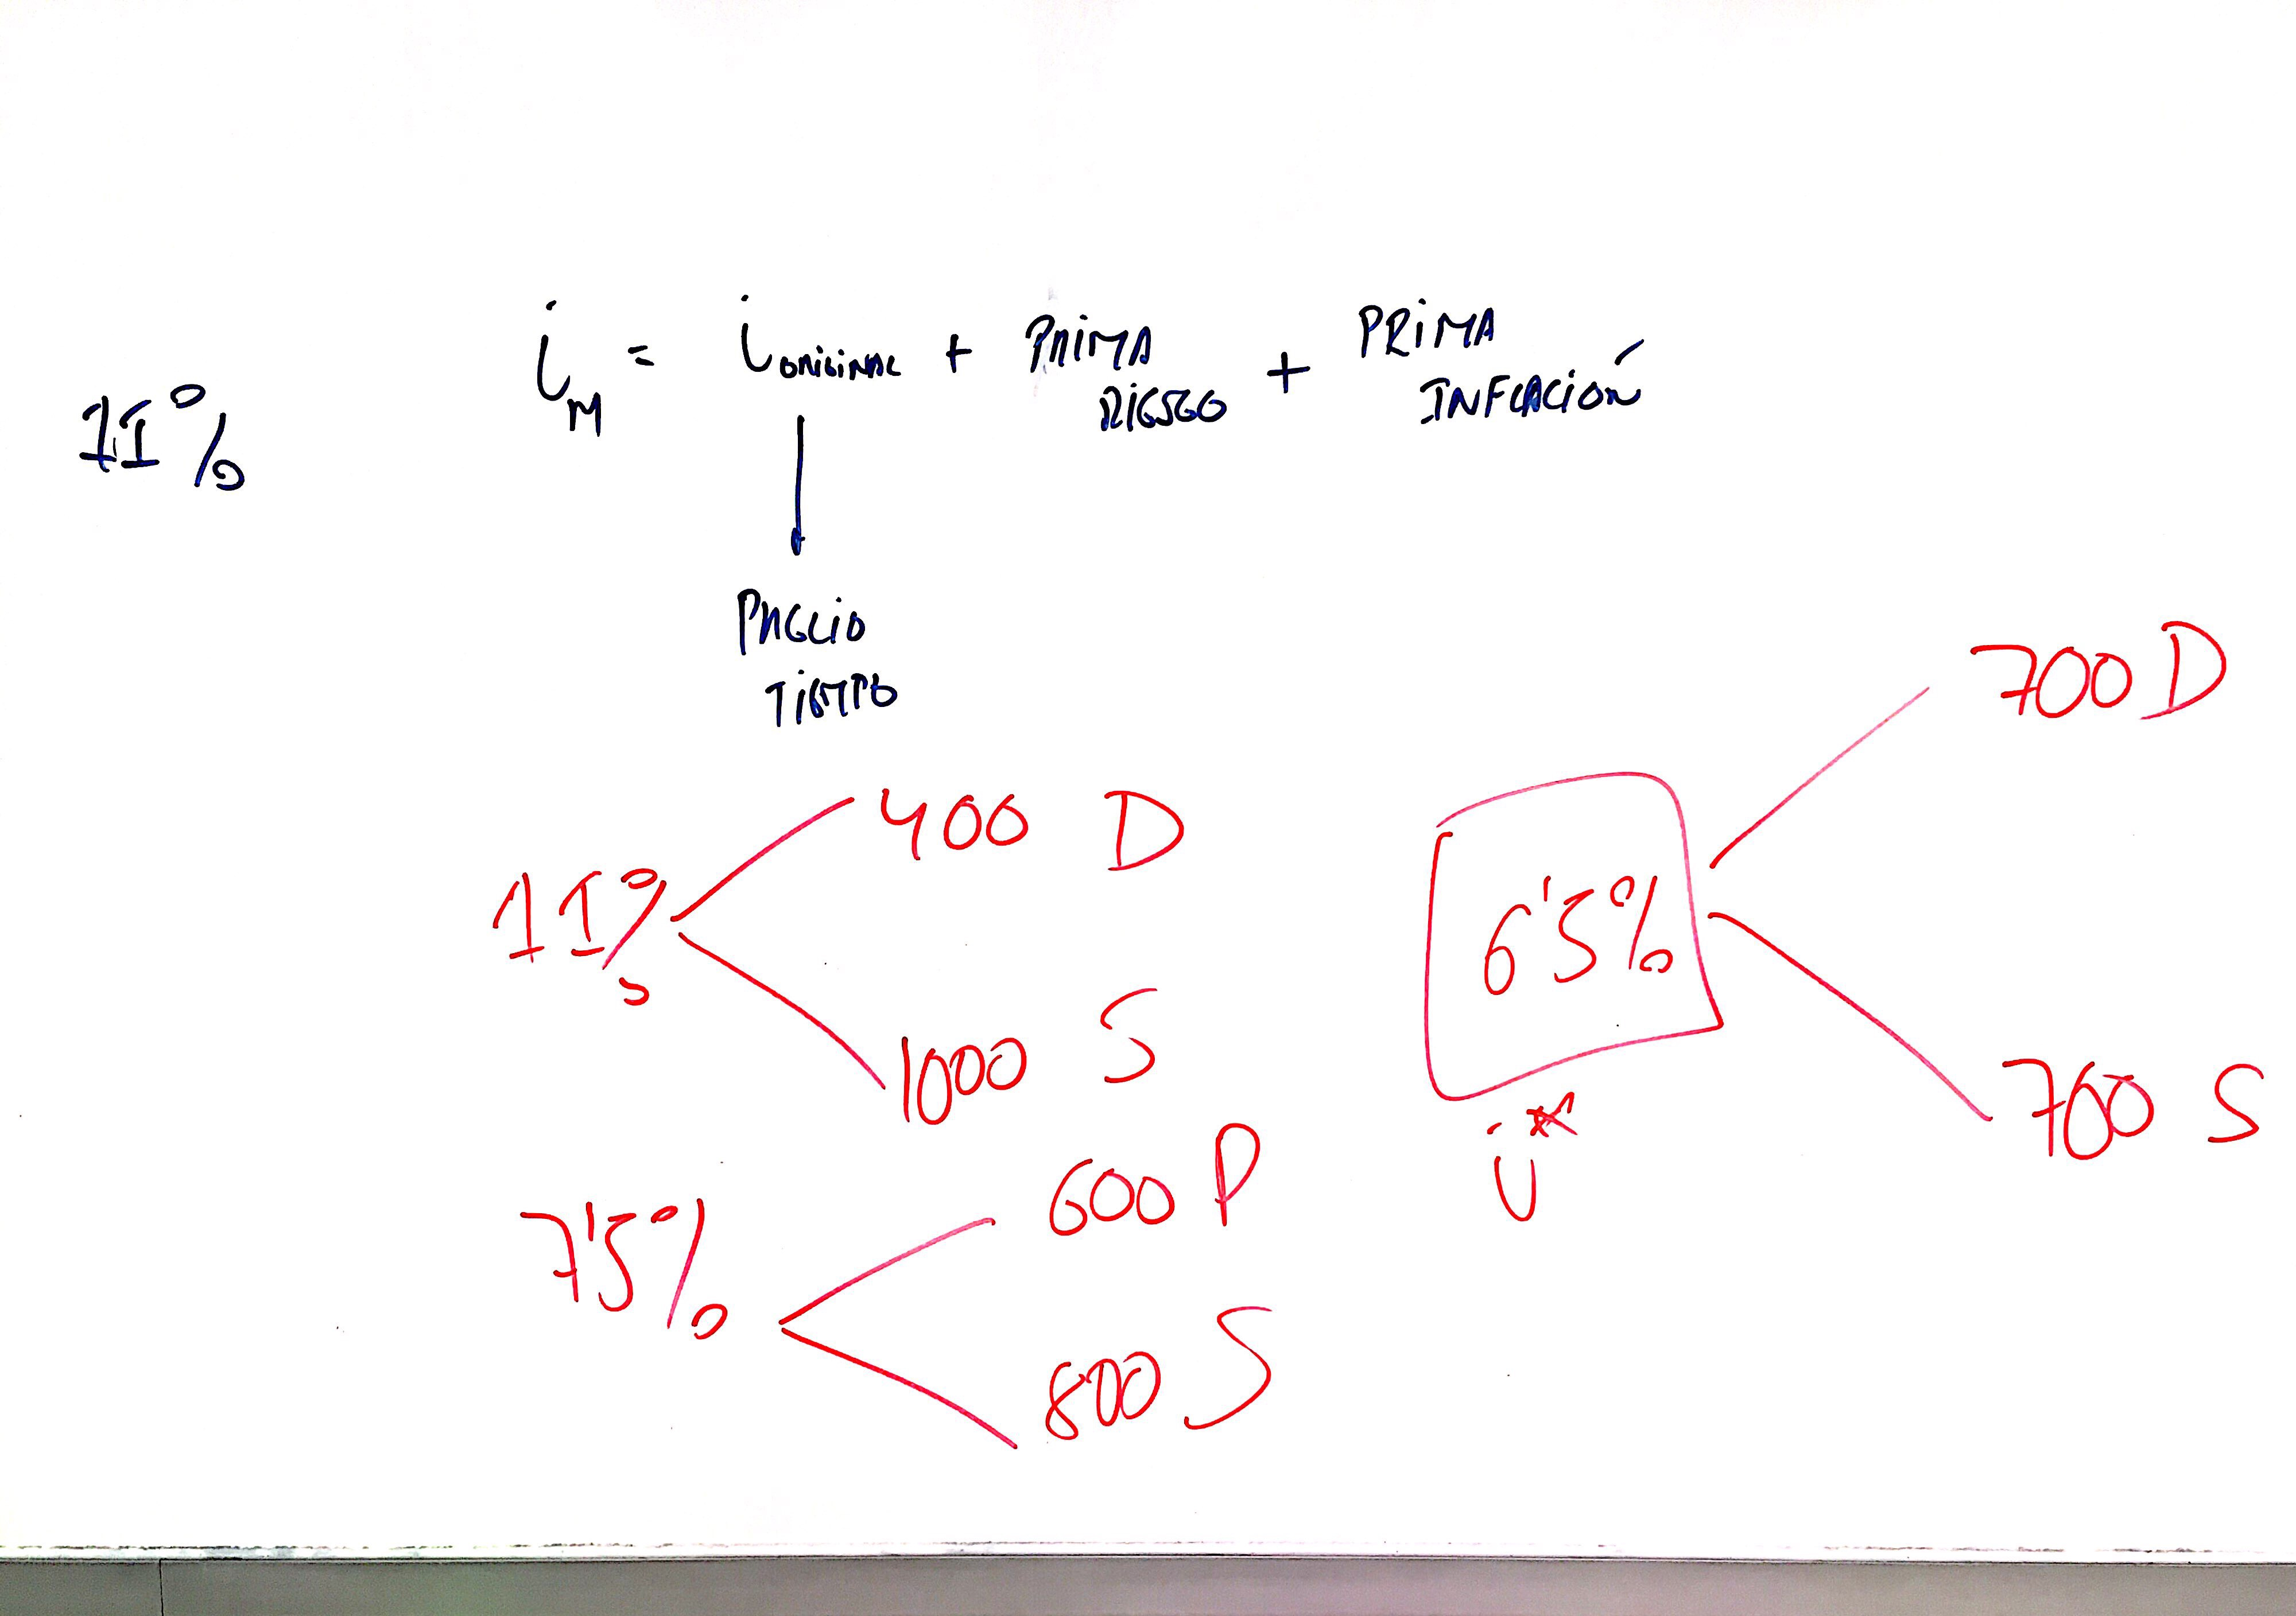
\includegraphics[width=6cm]{Classes/Images/2019-09-04-02.JPG}
    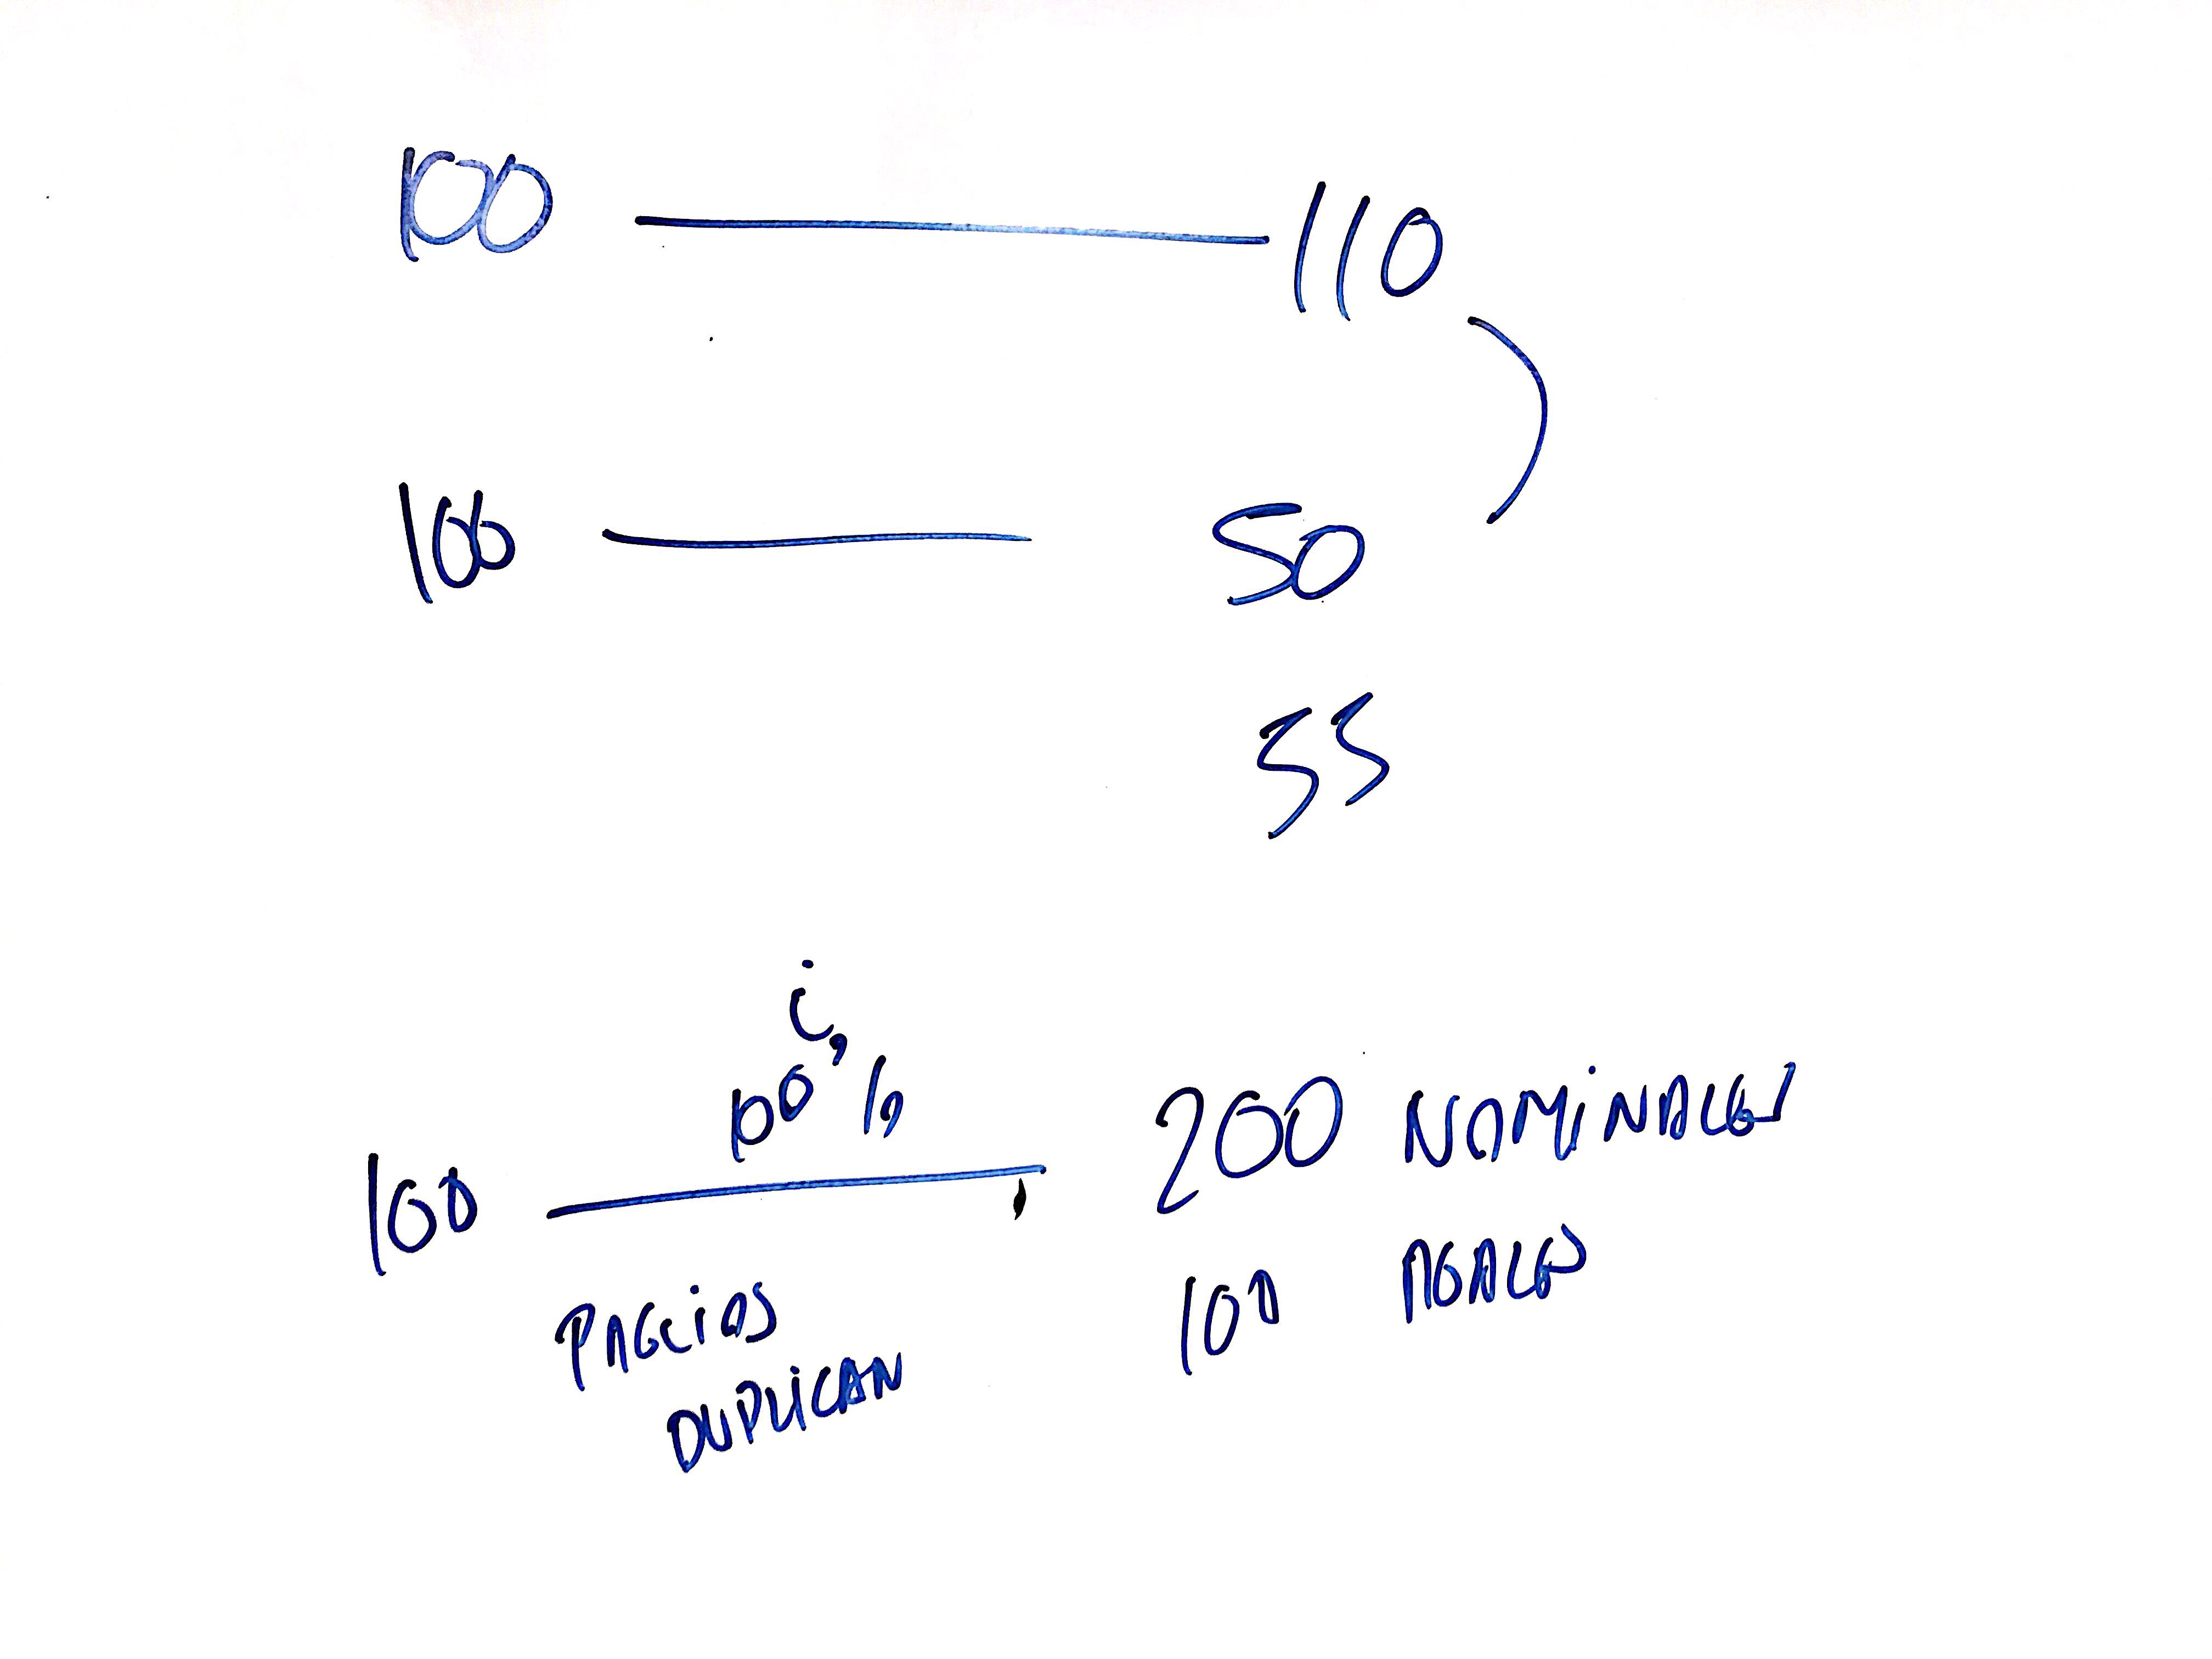
\includegraphics[width=6cm]{Classes/Images/2019-09-04-03.JPG}
    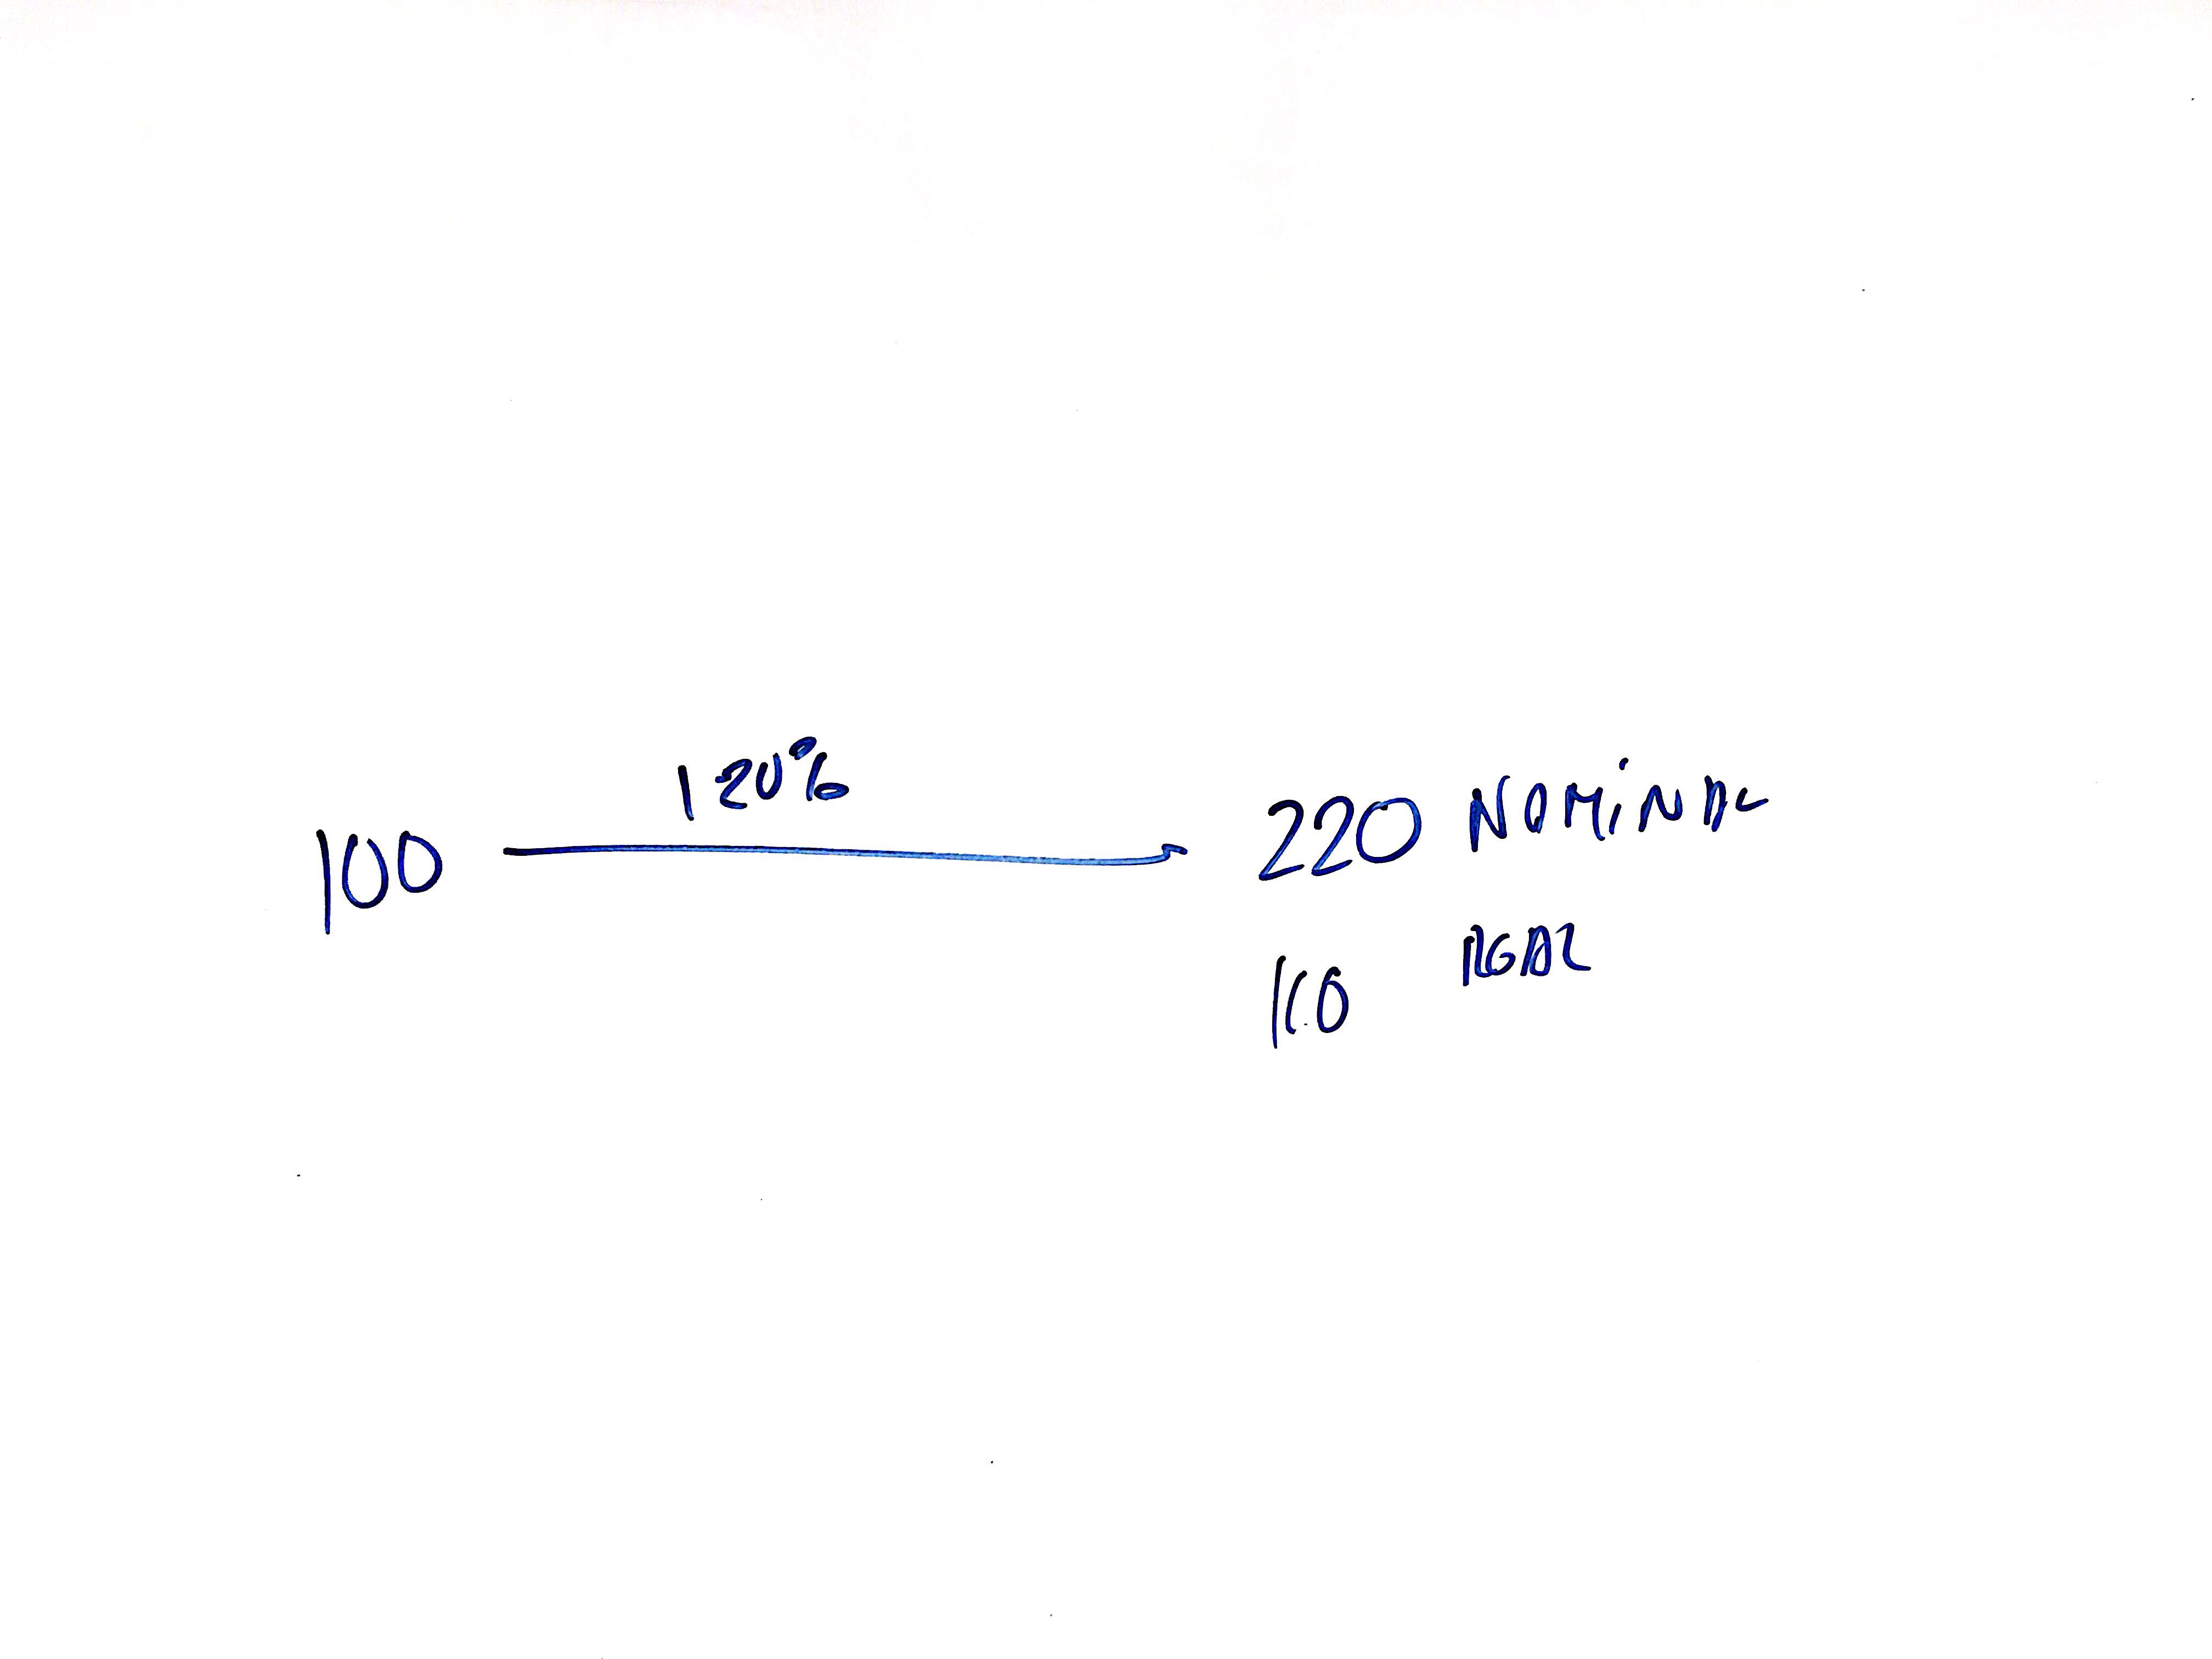
\includegraphics[width=6cm]{Classes/Images/2019-09-04-04.JPG}
    \caption{}
    \label{}
\end{figure} 

\begin{figure}[htbp]
    \centering
    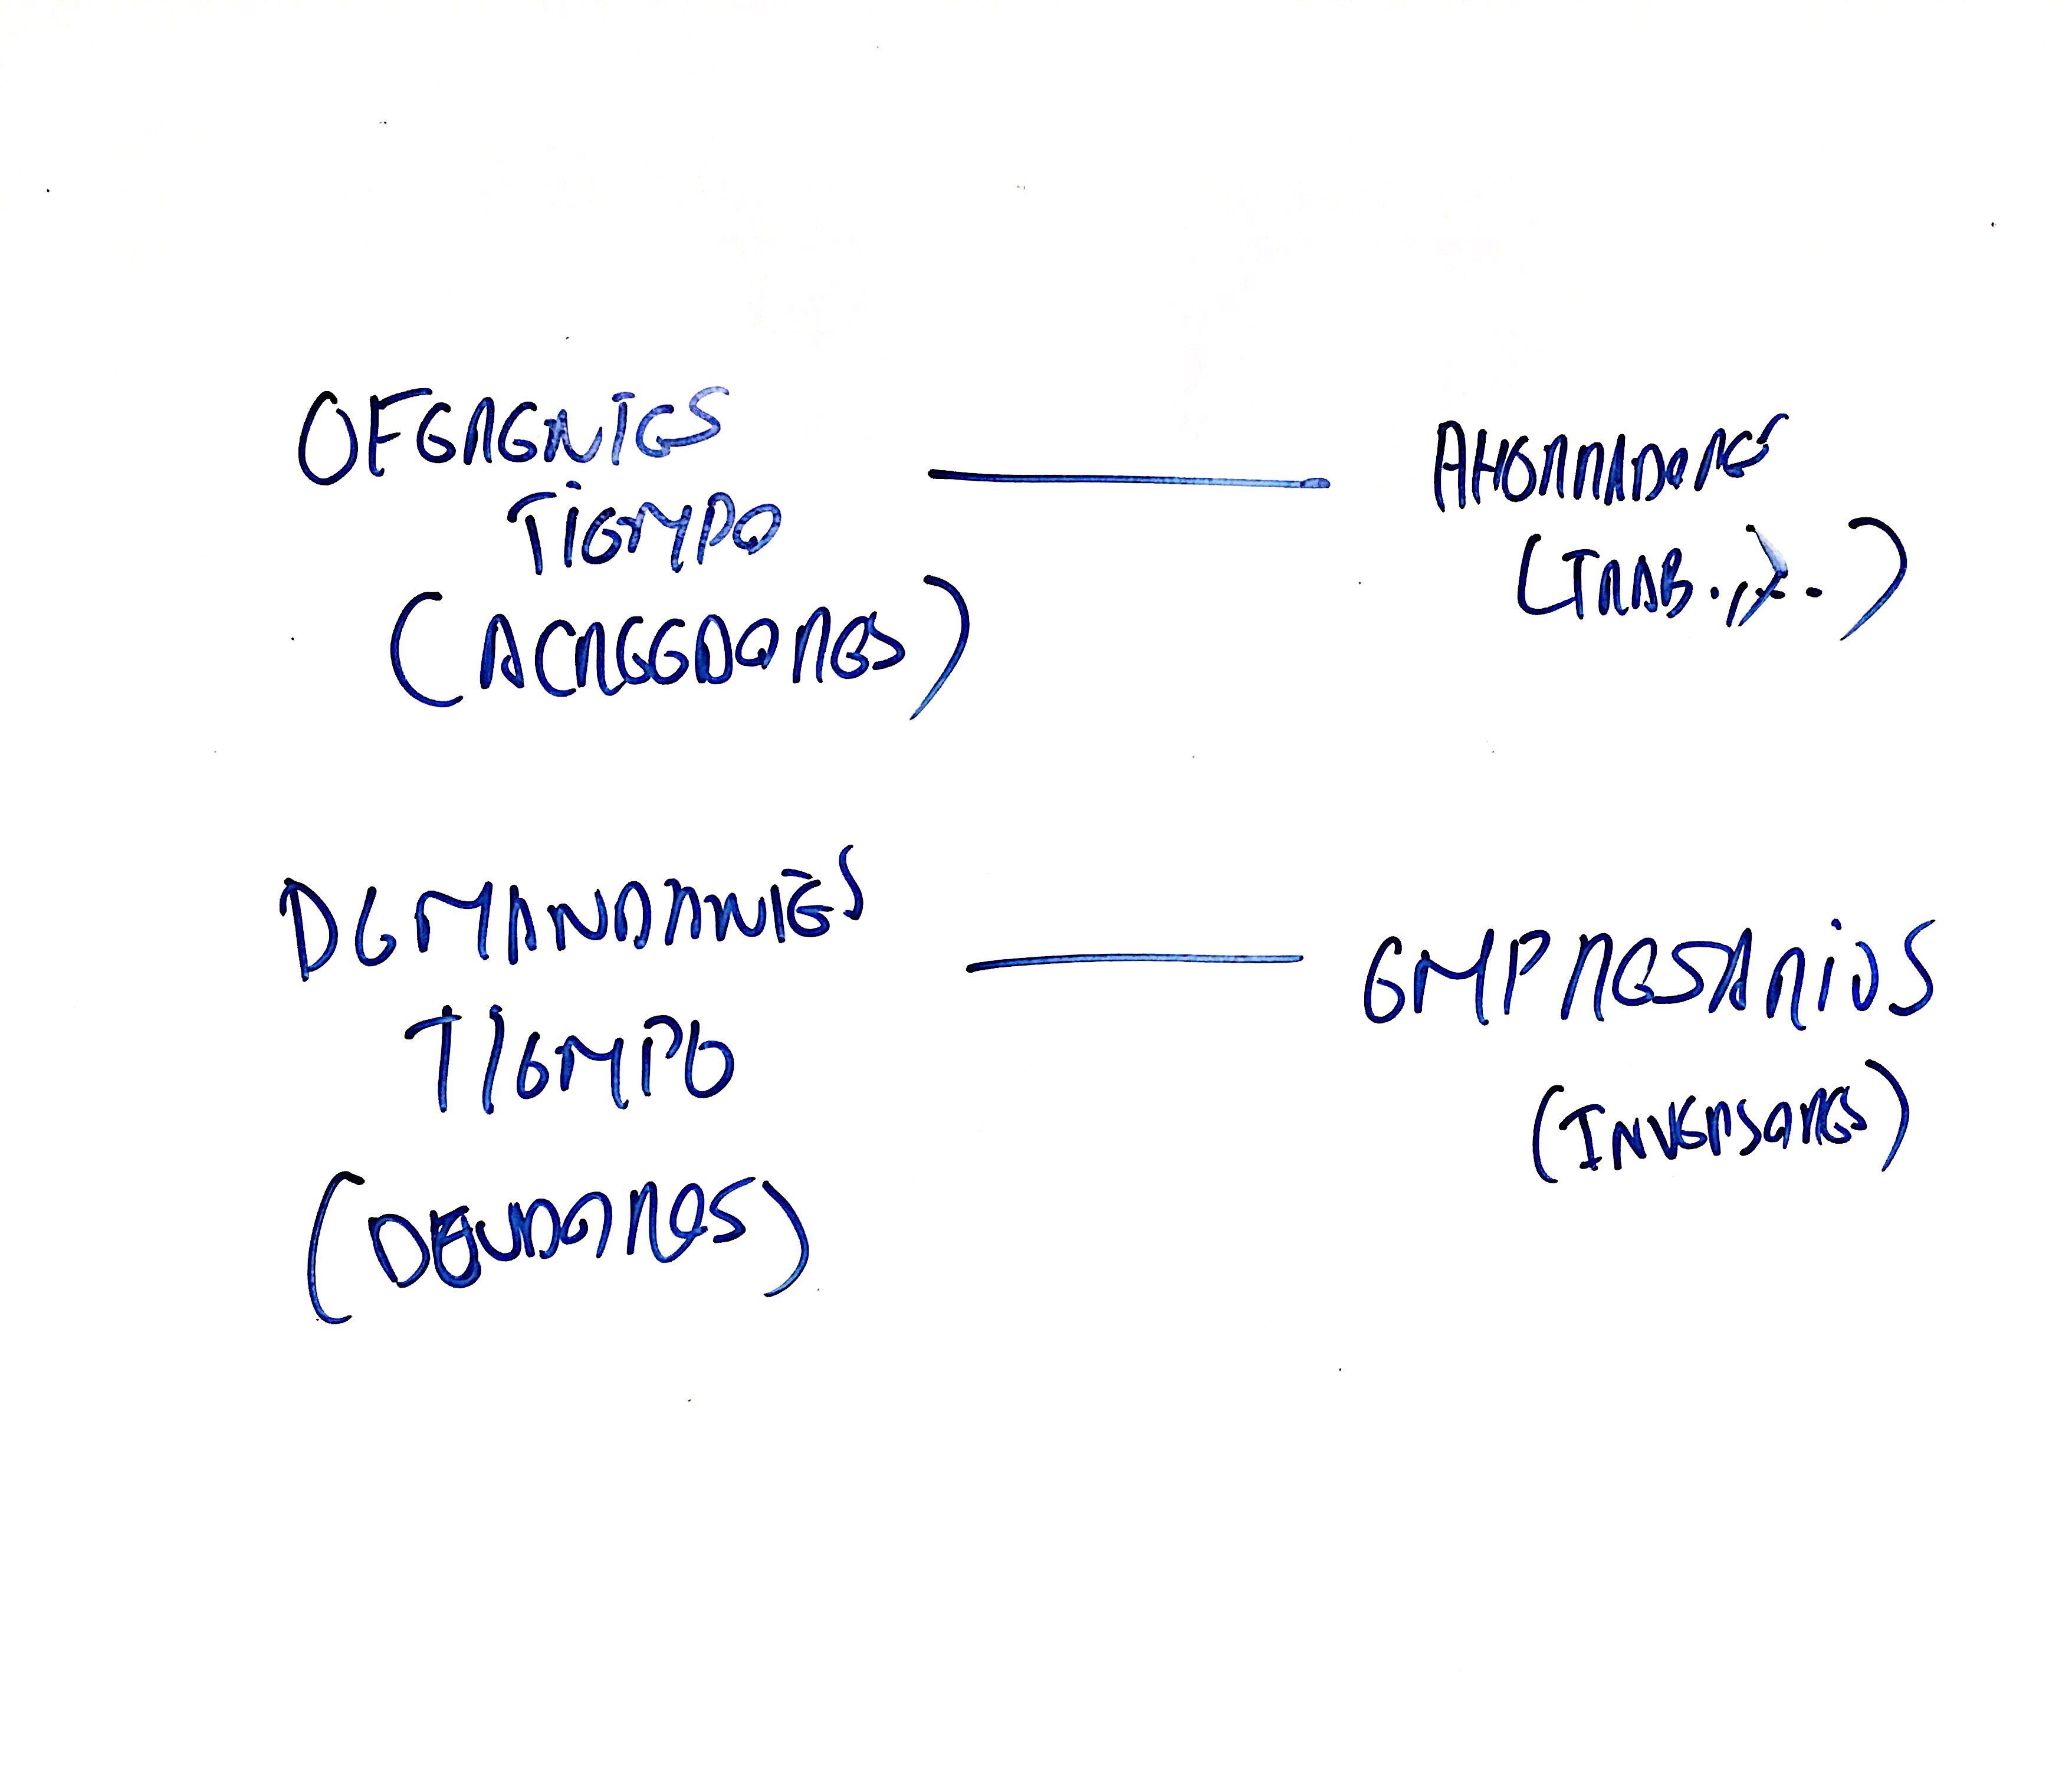
\includegraphics[width=6cm]{Classes/Images/2019-09-04-05.JPG}
    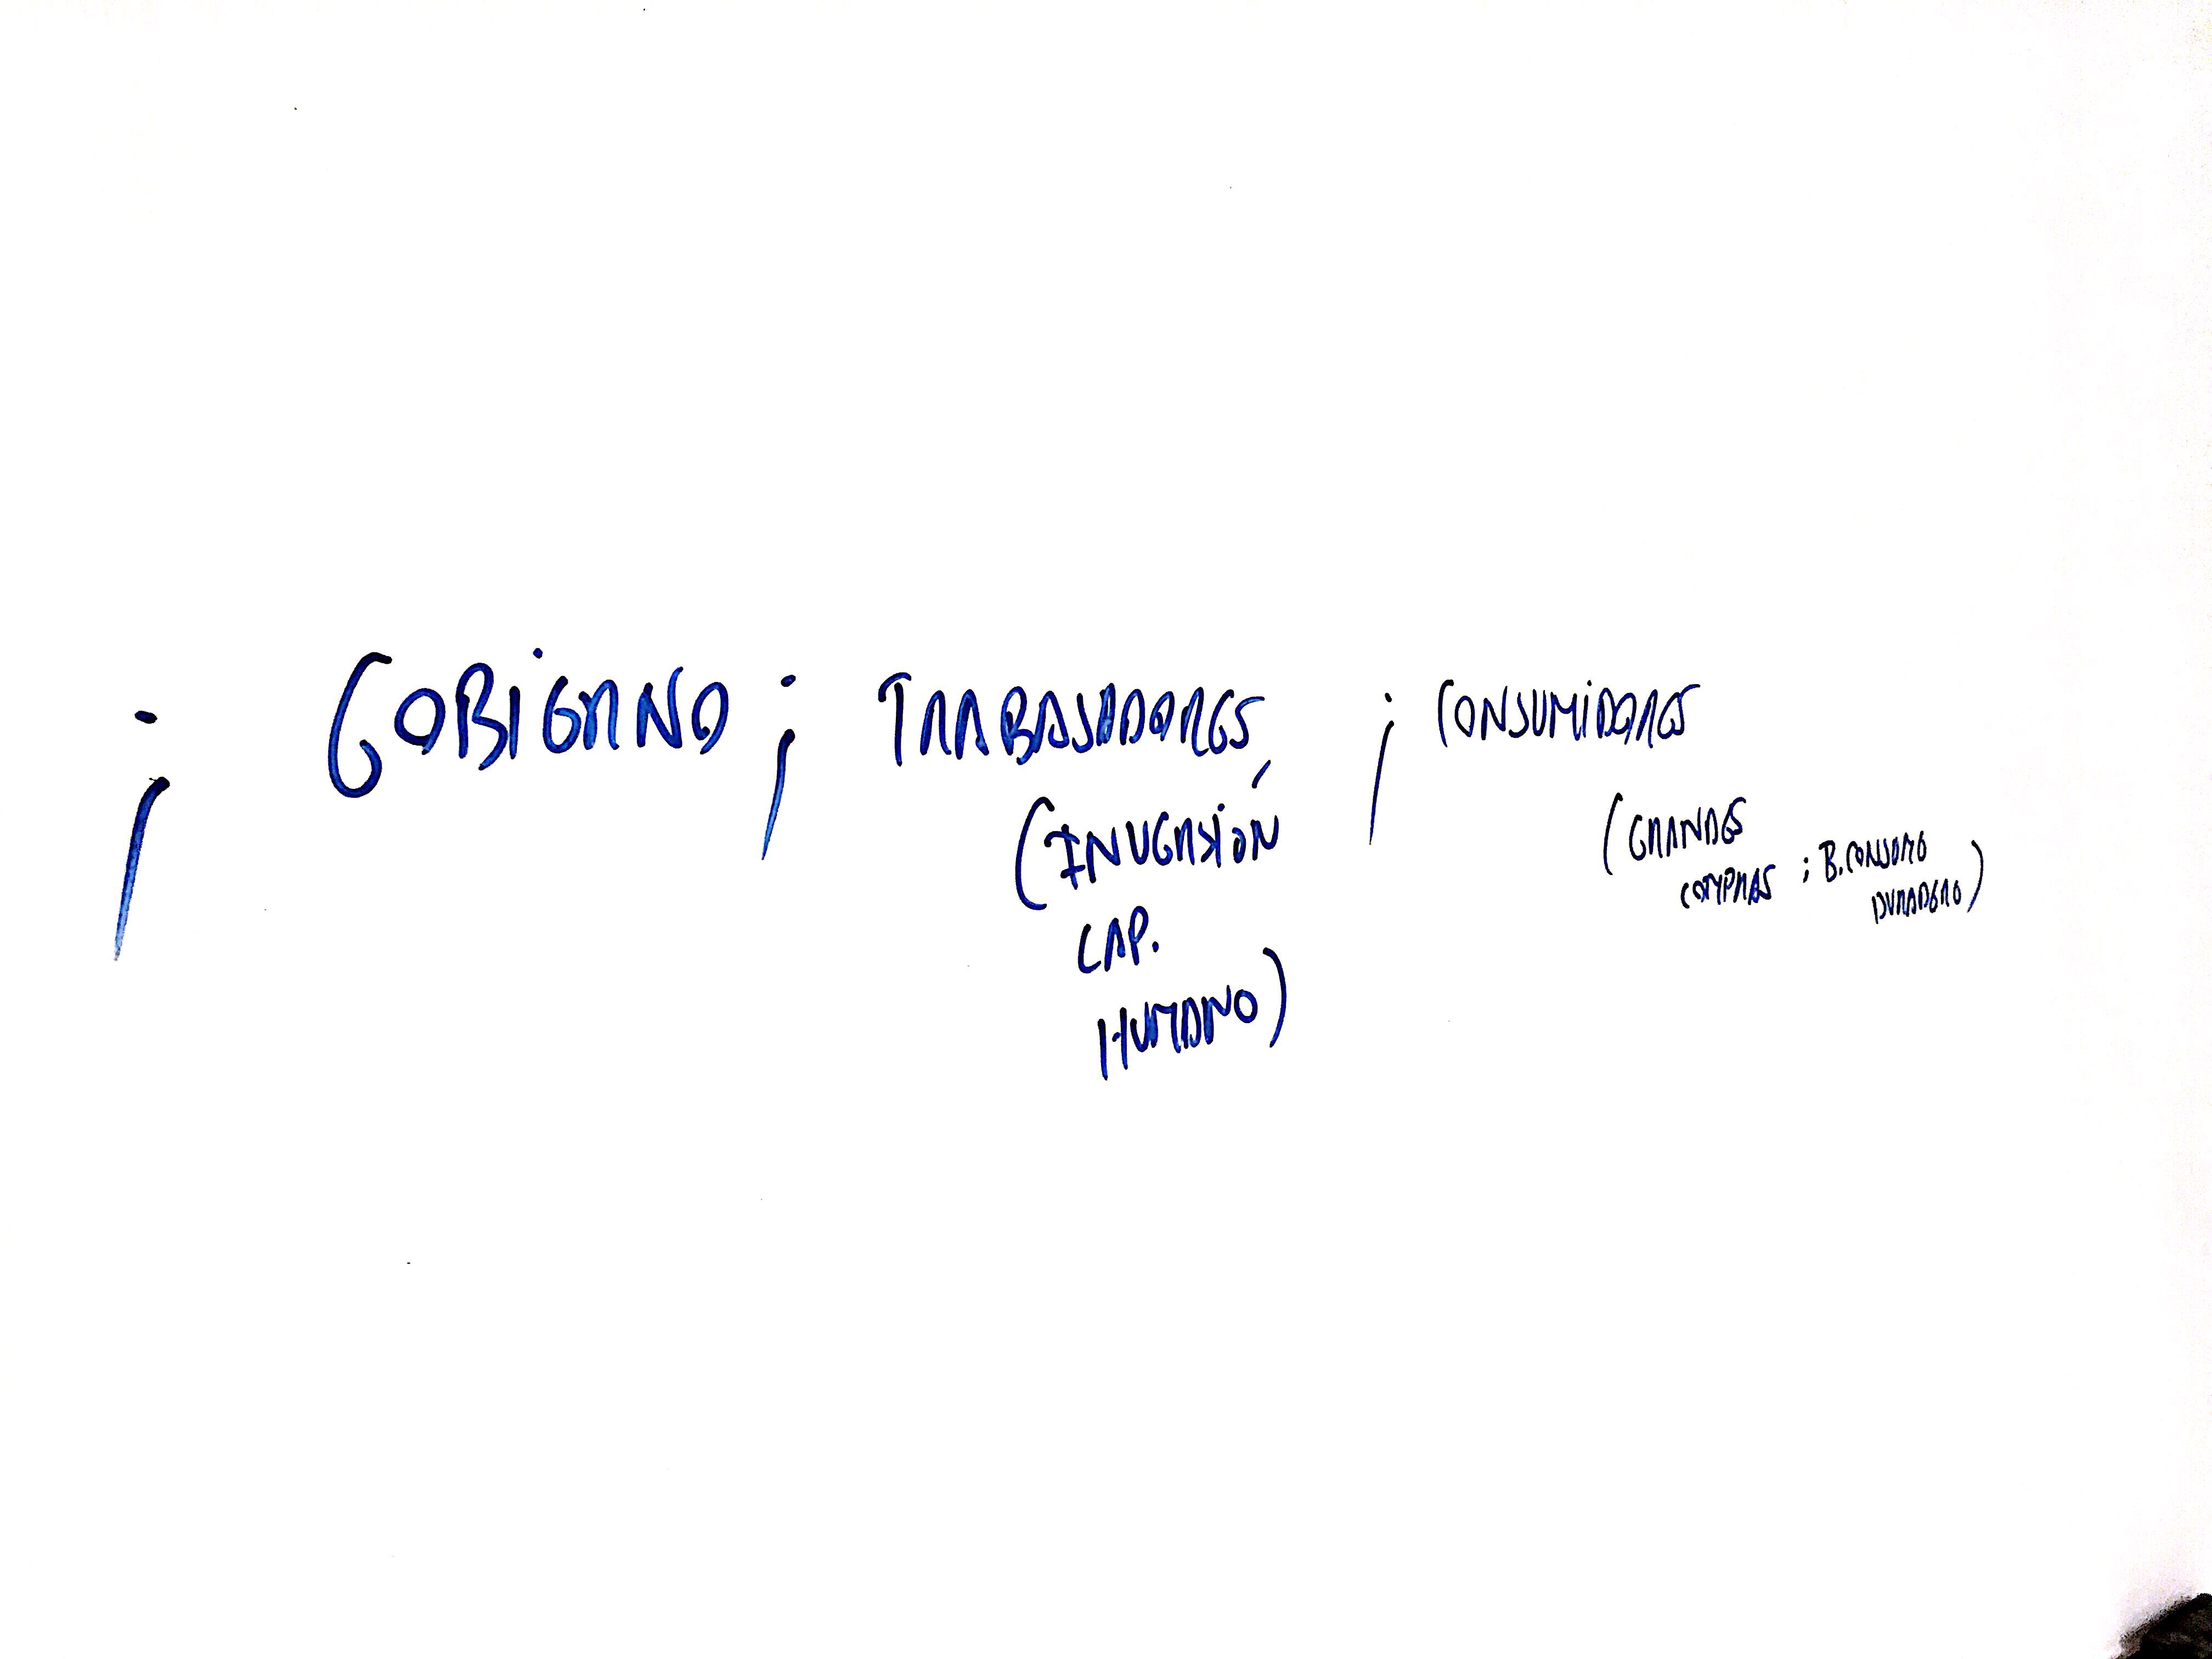
\includegraphics[width=6cm]{Classes/Images/2019-09-04-06.JPG}
    \caption{}
    \label{}
\end{figure} 


